\fontfamily{\sfdefault}\selectfont
% XCircuit output "aperture_noise2.tex" for LaTeX input from aperture_noise2.ps
\def\putbox#1#2#3#4{\makebox[0.00000in][l]{\makebox[#1][l]{}\raisebox{\baselineskip}[0.00000in][0.00000in]{\raisebox{#2}[0.00000in][0.00000in]{\scalebox{#3}{#4}}}}}
\def\rightbox#1{\makebox[0.00000in][r]{#1}}
\def\centbox#1{\makebox[0.00000in]{#1}}
\def\topbox#1{\raisebox{-0.60\baselineskip}[0.00000in][0.00000in]{#1}}
\def\midbox#1{\raisebox{-0.20\baselineskip}[0.00000in][0.00000in]{#1}}
   \scalebox{1}{
   \normalsize
   \parbox{5.65104in}{
   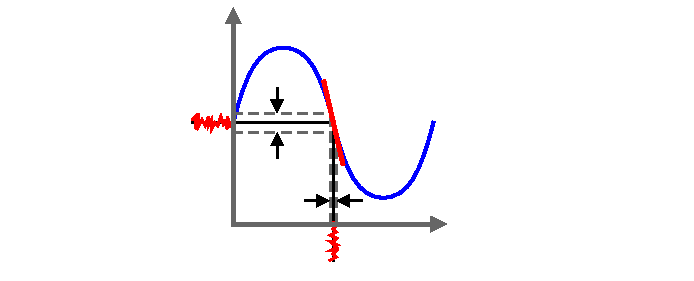
\includegraphics[scale=1.25000]{./figs/aperture_noise2.pdf}\\
   % translate x=96 y=256 scale 0.38
   \putbox{3.70000in}{0.31250in}{1.20}{\rotatebox{-360}{$t$}}%
   \putbox{1.66250in}{2.05000in}{1.20}{V}%
   \putbox{2.20000in}{1.68750in}{1.20}{$\sigma_{v}$}%
   \putbox{2.30000in}{0.65000in}{1.20}{$\sigma_{t}$}%
   \putbox{1.38750in}{1.57500in}{0.96}{Voltage }%
   \putbox{1.47500in}{1.45000in}{0.96}{noise}%
   \putbox{2.27500in}{0.30000in}{0.96}{Phase }%
   \putbox{2.30000in}{0.17500in}{0.96}{noise}%
   \putbox{1.36250in}{1.30000in}{1.20}{$\delta_{v}$}%
   \putbox{2.86250in}{0.12500in}{1.20}{$\delta_{t}$}%
   \putbox{2.82500in}{1.26250in}{1.80}{$\frac{dV}{dt}$}%
   } % close 'parbox'
   } % close 'scalebox'
   \vspace{-\baselineskip} % this is not necessary, but looks better
\fontfamily{\rmdefault}\selectfont
